% Chapter 5

\chapter{Diseño} % Main chapter title

\label{Chapter5} % Change X to a consecutive number; for referencing this chapter elsewhere, use \ref{ChapterX}

%Intro del capitulo
En este capítulo se propone el diseño de un simulador a nivel de sistema, para el cual se utilizó el análisis presentado en el capítulo anterior, de manera que las decisiones tomadas como resultado de tal análisis aquí aparecen asentadas para el diseño del simulador. El objetivo  de esta sección fue crear un modelo de sistema, para el cual se especificó el escenario que se implementará y el modelado de cuatro principales componentes que acabarán siendo implementados en el simulador: el despliegue de UEs, el modelo de canal, el esquema de acceso al múltiple al medio y los modelos de tráfico.\newline


%----------------------------------------------------------------------------------------
%	SECTION 
%----------------------------------------------------------------------------------------

\section{MODELO DE SISTEMA PROPUESTO}

Para empezar con el diseño de un simulador a nivel de sistema, se debe proponer un modelo de sistema que siga una norma o un modo determinado de operación, la gran parte de lo aquí planteado está fundamentado por aserciones hechas en diferentes publicaciones científicas, primordialmente de artículos de revistas IEEE.

En primera instancia se comenzó con la etapa de análisis (\textit{Capítulo \ref{Chapter4}}), donde se analizaron los requisitos de la red, las características que debía tener el escenario que se propondría después y los distintos modelos que formarán parte de la simulación. Todo esto en el contexto de una red celular 5G que brinde servicio a nodos IoT.

En términos generales, se considerará una red celular uni-celda para transmisiones de subida (\textit{uplink}), el escenario se trata de uno urbano micro celular (UMi) en donde frecuentemente los UEs se encuentran estáticos y en el exterior. De acuerdo a los modelos analizados y ya elegidos en el \textit{Capítulo \ref{Chapter4}}, el modelo de sistema del simulador se concentrará en la implementación de los siguientes sub-sistemas \textit{[Figura~\ref{fig:DiagramaGral}]}:

\begin{enumerate}
    \item  Uso de una geometría estocástica, es decir, despliegue de UEs siguiendo un PPP \textit{(Sección }.
    \item  Pérdidas de canal usando un modelo CI para ambientes exteriores \textit{(Sección }.
    \item  Incorporación de un esquema de acceso al medio no ortogonal (NOMA) usando una técnica de agrupamiento \textit{(clustering)} de usuarios \textit{(Sección }.
    \item  Diferentes modelos de tráfico que simulen distintos servicios para NB-IoT \textit{(Sección }.
\end{enumerate}

El simulador está enfocado en el caso de uso de mMTC (o mIoT) el cual se caracteriza por brindar servicio a un gran número de dispositivos, esto es, teniendo una alta densidad de volumen de tráfico en escenarios con aglomeración de dispositivos. Por lo tanto, como se revisó en la \textit{Seccion } un excelente candidato para cumplir con los requerimientos del caso de uso mIoT y que forma ahora parte del estándar 5G, es la tecnología NB-IoT. De este estándar, se tomarán sus especificaciones técnicas (\textit{Sección }), tales como los parámetros fundamentales para la comunicación entre la BS y los UEs en la simulación.\newline

De acuerdo con lo revisado en tres artículos del Capítulo \ref{Chapter3} del Estado del Arte \parencite{Kouzayha2018} \parencite{Zhang2017} \parencite{Shahini2019} donde se estudiaron modelos de sistema orientados al análisis de PD-NOMA, vemos que una geometría estocástica con distribución de BSs y UEs usando PPP es ampliamente utilizada, porque sirven como modelo de referencia para redes masivas y de interferencia limitada. Acerca del canal, los tres artículos coinciden en caracterizar las perdidas por medio de un exponente de pérdida y un desvanecimiento plano tipo Rayleigh siguiendo una distribución exponencial con media 1, lo cual es un canal comúnmente considerado en este tipo de escenarios. Además, al considerar sistemas limitados en interferencia proponen un factor de reúso de 1, se hace gran énfasis en los cálculos de interferencias intercelulares y sus efectos en el rendimiento. Partiendo de estas premisas se propone el Modelado de los primeros 3 módulos del simulador:

\begin{figure}[th]
    \centering
    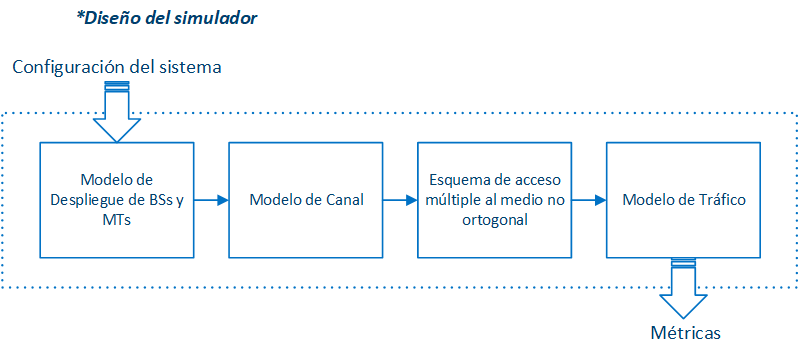
\includegraphics[scale=1]{Figures/Diagrama general de bloques del simulador}
    \decoRule
    \caption[Diagrama general de bloques del simulador, constando principalmente de 4 módulos.]{Diagrama general de bloques del simulador, constando principalmente de 4 módulos.}
    \label{fig:DiagramaGral}
\end{figure}

A continuación se definen las características generales de cada sub-sistema:\newline

\subsection{Uso de una geometría estocástica, es decir, despliegue de UEs siguiendo un PPP}

De igual manera que como se realizó en \parencite{Kouzayha2018} y \parencite{Zhang2017} con el fin de obtener un análisis fundamental, se propone la generación de una geometría estocástica en 2D para la distribución de nodos. Se toma como modelo de despliegue un \textit{Poisson Point Process }(proceso puntual de Poisson, PPP) con distintas densidades de dispositivos para la asignación espacial de los nodos IoT. El hecho de considerar dos clases de nodos, es decir, clase 1 y clase 2, se buscará que por cada nodo de clase 2 hayan por lo menos 3 nodos de clase 1. por lo tanto se utilizarán diferentes tasas para la generación de estos nodos. \newline

\subsection{Pérdidas de canal usando un modelo CI para ambientes exteriores}

En la \textit{Sección } se establecieron las aplicaciones de los diferentes dominios de IoT que se utilizarán para la implementación del simulador. Todas estas aplicaciones se encuentran presentes, no exclusivamente pero sí particularmente, en escenarios urbanos y en exteriores, por lo tanto se implementará el Modelo CI (Secc. ) el cual de acuerdo a lo estudiado en \parencite{Sun2016} es el modelo que mejor estima la señal en este tipo de ambientes. Además, se agregarán perdidas por el desvanecimiento rápido, usando el modelo de desvanecimiento de Rayleigh (siguiendo una distribución exponencial con media 1 y que se distribuya de forma independiente e idéntica [i.i.d.]), este es ideal para entornos urbanos en situaciones donde hay un gran número de multi-trayectorias de la señal y reflexiones causadas por los edificios y objetos que obstruyen la línea de vista. \newline

\subsection{Incorporación de un esquema de acceso al medio no ortogonal (NOMA) usando una técnica de agrupamiento de usuarios}

Se predefine que existirá un bloque de recursos (PRB) para un eNB dedicado para comunicaciones tipo maquina (MTC) utilizando el estándar NB-IoT. El recurso de radio será una banda de frecuencias de 180kHz. Esta banda se dividirá en 48 sub-bandas de 3.75kHz.\newline

Por lo tanto, para la compartición de recursos, en vías de dar servicio a un gran número de dispositivos, se propone la implementación de un esquema de acceso múltiple al medio no ortogonal (NOMA) descrito en la \textit{Sección } y la implementación de una técnica de agrupamiento de usuarios (revisada en \textit{Sección }) y se aprovechará la no ortogonalidad, para agrupar diferentes clases de nodos IoT en una misma sub-banda. \newline

\subsection{Diferentes modelos de tráfico que simulen distintos servicios para NB-IoT}

En la implementación de modelos de tráfico se tendrá en cuenta el modelo CMMPP y un modelo determinístico. El modelo CMMPP tendrá una implementación distinta para cada una de las aplicaciones que proponemos en la \textit{Tabla~\ref{tab:} } a excepción de aquellas aplicaciones con tasas de transmisión periódicas, para las cuales se utilizará un modelo determinístico\textit{.} Cada una de las implementaciones del modelo CMMPP tendrá su propio diseño de cadena de Markov con distintas tasas de generación de paquetes por estado, las cuales dependerán de la aplicación, además, cada implementación contará con su propia matriz de transición entre estados. Esto se debe a que la relación espacial y temporal que existe entre los nodos a la hora de transmitir dependerá del tipo de aplicación.

Cada nodo, al tener su propia cadena de Markov (la que determinará su estado en cada momento) contará con tres procesos (uno por cada aplicación con tráfico aleatorio), llamados \textit{procesos maestros}. Estos procesos, uno por cada aplicación con tráfico aleatorio, estarán modificando las probabilidades de cambio de estado de cada nodo según su proximidad a otros nodos que estén cambiando de estado. Por ejemplo, digamos que un nodo, que llamaremos N1, que detecta terremotos se encuentra en estado de reposo y su probabilidad de transición al estado de transmisión por un evento es del 1\%, ahora de pronto otro nodo (de la misma aplicación) en su proximidad cambia de estado a transmisión por evento, y unos instantes después la probabilidad de transición en nuestro nodo muestra que antes era del 1\% aumenta hasta 90\%, lo que desencadena que este nodo también comience a transmitir al cambiar de estado unos momentos después. El ejemplo anterior, en la vida real se traduciría como un terremoto ocurriendo en un lugar y una gran cantidad de nodos que se encargan de detectarlo comenzando de pronto a transmitir con una indudable coordinación espacial y temporal.

\begin{figure}[th]
\centering
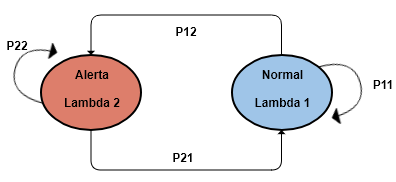
\includegraphics[scale=1]{Figures/Cadena de Markov propuesta}
\decoRule
\caption[Cadena de Markov propuesta]{Cadena de Markov propuesta}
\label{fig:CMMPPpropuesta}
\end{figure}

Habiendo explicado esto, la implementación del modelo CMPP en las aplicaciones, control de iluminación, detección de terremotos y genérico contará con un diseño de cadena de Markov como el que se presenta en la \textit{Figura~\ref{fig:}. }En esta figura se puede ver que se modelarán dos distintos estados para cada nodo IoT de estas aplicaciones. El primer estado, llamado normal corresponde al funcionamiento \textbf{normal} o principal de la aplicación, con una tasa de transmisión Lambda 1 (${\lambda }_1$), mientras que el segundo estado, llamado \textbf{Alerta} con tasa de transmisión Lambda 2 (${\lambda }_2$), este último corresponde al estado que acudirán los dispositivos IoT de acuerdo con eventos producidos aleatoriamente con base en la aplicación del nodo. Es justamente con la ayuda de este estado que el modelo será capaz de simular la coordinación espacial y temporal de los dispositivos. Otro componente clave del modelo CMMPP es la matriz $P_n$, la cual contiene las probabilidades de cambio de estado que se pueden apreciar en la \textit{Figura~\ref{fig:}}. Esta matriz se encontrará modulada por un proceso distinto para cada aplicación de la siguiente forma:

\begin{equation}
P_n\left[k\right]=\ _n\left[k\right] P_c+\left(1-\ _n\left[k\right]\right)\ P_u 
\label{eqn:Pn}
\end{equation}

\[donde:\ n\ corresponde\ al\ n-\textrm{é}simo\ nodo\] 
\[y\ k\ a\ un\ determinado\ instante\ de\ tiempo\] 

En la ecuación \ref{eqn:Pn} vemos la forma en la que se modulan las matrices de probabilidad de transición entre los estados. Entonces para calcular la matriz $P_n\left[k\right]$, es decir la perteneciente al nodo \textit{n }en el instante \textit{k, }necesitamos de las matrices $P_c$ y $P_u$ que corresponden al comportamiento coordinado y no coordinado respectivamente y del valor $_n\left[k\right]$. Comenzaremos con las matrices $P_c$ y $P_u$, estas matrices marcan el comportamiento que tendría el nodo en los casos extremos de coordinación o en la ausencia de esta, esto debido a que $_n\left[k\right]$.varía entre [0 ,1], entonces si existe una perfecta coordinación entre nodos y este valor es 1, en algún momento, el segundo sumando de la ecuación \ref{eqn:Pn} sería 0 y $P_n\left[k\right]=\ P_c$. La propuesta inicial para $P_c$ y $P_u$ es la siguiente, tal y como se ha utilizado en \parencite{Gupta2018} y \parencite{Smiljkovic2014}:

\begin{equation}
P_{u} =  
\begin{bmatrix}
1 & 1 \\
0 & 0 
\end{bmatrix}
\end{equation}

\begin{equation}
P_{c} = 
\begin{bmatrix}
0 & 1 \\
1 & 0 
\end{bmatrix}
\end{equation}

Ahora se estudia el término $_n\left[k\right]$ que es el que se encarga de simular la correlación existente entre los nodos, el cual se compone de $_n\left[k\right]=\ {\delta }_n[k]$, siendo ${\delta }_n$ el término encargado de la coordinación espacial y $[k]$ el de la coordinación temporal. Para ${\delta }_n$ se utilizarán dos distribuciones: una exponencial decreciente y una ventana de coseno alzado según convenga para la aplicación tal y como se propone en \parencite{Gupta2018}, la posibilidad de implementar la ventana de coseno alzado es por el efecto de un término abrupto que puede simular, lo que evitaría el problema de inundación de tráfico por un incorrecto diseño. Finalmente para $[k]$ se tiene una variable aleatoria beta\textit{ }que simulará la correlación temporal. \newline

Mientras un nodo se encuentre en un estado, este generará paquetes a la tasa $\lambda$ marcada en ese estado específico. Un cambio de estado se dará ya sea por la influencia de otro nodo vecino o por un cambio originado en el mismo nodo, esto último en el mundo real se traduciría a que este nodo es el primero en detectar el evento y cambiarse al estado de alarma, lo que desencadenaría que otros nodos posiblemente de igual manera cambien su comportamiento. En la \textit{Figura~\ref{fig:CMMPP_Algoritmo}} se presenta el diagrama de flujo que las distintas realizaciones del modelo CMMPP desarollarán en la simulación.\newline

\begin{figure}[th]
\centering
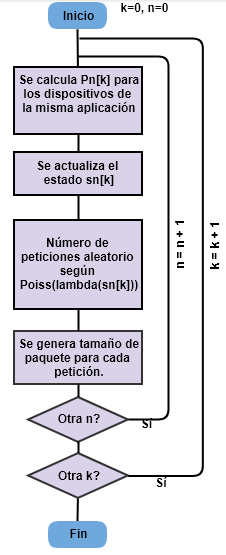
\includegraphics[scale=.7]{Figures/Generación de tráfico con modelo CMMPP}
\decoRule
\caption[Generación de tráfico con modelo CMMPP]{Generación de tráfico con modelo CMMPP}
\label{fig:CMMPP_Algoritmo}
\end{figure}

El segundo modelo se trata de uno determinístico, y será el que se implementará en las aplicaciones cuya tasa de tráfico es periódica. De manera que lo único que se debe conocer es la tasa de tráfico de los nodos y poner un temporizador en cada uno, con la finalidad de que cuando acabe, éste genere un evento de transmisión. Las aplicaciones contempladas para este modelo son: el monitoreo del consumo de agua y electricidad en la ciudad, el monitoreo de la contaminación del aire y el control dinámico de los semáforos.\newline


\begin{table}
\caption{Caracterización de las aplicaciones seleccionadas}
\label{tab:AppsSimulacion}
\centering
\begin{tabular}{|p{1.4in}|p{0.7in}|p{0.7in}|p{0.7in}|p{0.4in}|p{1.8in}|} \\ 
\textbf{\textit{Número de Servicio y Nombre}} & \textbf{Tamaño de red} & \textbf{Tasa de tráfico} & \textbf{Demanda de QoS} & \textbf{Clase} & \textbf{Tamaño de paquete} \\ 
\textit{1 - Control de iluminación\newline (Ciudad Inteligente) } & \footnotesize{ Grande, miles de dispositivos } & \footnotesize{ Aleatorio, poco frecuente } & \footnotesize{ Media, tolerante al retardo 15seg } & \footnotesize{ 1 } & \footnotesize{ Activación aleatoria\newline \textbf{UL}: 20 bytes \textit{payload}\newline \textbf{DL}: ACK de 0 bytes } \\ \hline 
\textit{2 - Monitoreo del consumo de agua y electricidad en la ciudad\newline (Ciudad Inteligente) } & \footnotesize{ Media a grande, cientos a miles de dispositivos } & \footnotesize{ Periódico, 1 msj cada 10 min por dispositivo } & \footnotesize{ Baja, tolerante al retardo 1min } & \footnotesize{ 1 } & \footnotesize{ Activación periódica\newline \textbf{UL}: distribución de Pareto con parámetro alfa = 2.5 y tamaño mínimo de carga útil de la aplicación = 20 bytes con un corte a 200 bytes\newline \textbf{DL}: ACK de 0 bytes 50\% de las veces. } \\ \hline 
\textit{3 - Detección de terremotos\newline (Ambiente Inteligente) } & \footnotesize{ Media a grande, cientos a miles de dispositivos } & \footnotesize{ Aleatorio, poco frecuente } & \footnotesize{ Alta, tolerante al retardo 3seg } & \footnotesize{ 1 } & \footnotesize{ Activación aleatoria\newline \textbf{UL}: 20 bytes \textit{payload}\newline \textbf{DL}: ACK de 0 bytes } \\ \hline 
\textit{4 - Monitoreo de contaminación del aire\newline (Ambiente Inteligente) } & \footnotesize{ Media a grande, cientos a miles de dispositivos } & \footnotesize{ Periódico, 1 msj cada 15 min por dispositivo } & \footnotesize{ Media, tolerante al retardo 15seg } & \footnotesize{ 1 } & \footnotesize{ Activación periódica\newline \textbf{UL}: distribución de Pareto con parámetro alfa = 2.5 y tamaño mínimo de carga útil de la aplicación = 20 bytes con un corte a 200 bytes\newline \textbf{DL}: ACK de 0 bytes 50\% de las veces. } \\ \hline 
\textit{5 - Control dinámico de semáforos\newline (Transporte y Movilidad Inteligentes) } & \footnotesize{ Grande, miles de dispositivos } & \footnotesize{ Periódico, 1 msj cada min por dispositivo } & \footnotesize{ Alta, tolerante al retardo 5seg } & \footnotesize{ 1 } & \footnotesize{ Activación periódica\newline \textbf{UL}: distribución de Pareto con parámetro alfa = 2.5 y tamaño mínimo de carga útil de la aplicación = 20 bytes con un corte a 200 bytes\newline \textbf{DL}: ACK de 0 bytes 50\% de las veces. } \\ \hline 
\textit{6 - Genérico}  & \footnotesize{ Grande, miles de dispositivos } & \footnotesize{ Aleatorio, poco frecuente } & \footnotesize{ Alta, tiempo real } & \footnotesize{ 2 } & \footnotesize{ Activación aleatoria\newline \textbf{UL}: 20 bytes \textit{payload}\newline \textbf{DL}: ACK de 0 bytes } \\ 
\end{tabular}
\end{table}

Ahora, en la \textit{Tabla~\ref{tab:AppsSimulacion}} se presentan las aplicaciones mencionadas en la \textit{sección } junto a su caracterización. Adicionalmente se anexa la distinción de las aplicaciones en dos clases distintas, lo que permitirá implementar el agrupamiento de los dispositivos para que compartan recursos en un esquema NOMA.

También, en la \textit{Tabla~\ref{tab:AppsSimulacion}} se puede ver que para las transmisiones de bajada (\textit{downlink}) se componen de simples confirmaciones de llegadas (ACK) de paquetes de longitud 0 (\textit{bytes)}, es la razón por la que se limitó el análisis a un estudio del el enlace de subida (\textit{uplink}). En el enlace de subida, solo se considerará la interferencia intracelular, proveniente de los UE que compartan un mismo grupo (\textit{cluster}).

En la \textit{Figura~\ref{fig:EscenarioMTC}} se plantea una aproximación del escenario mMTC descrito, usando un agrupamiento con cuatro nodos.

\begin{figure}[th]
\centering
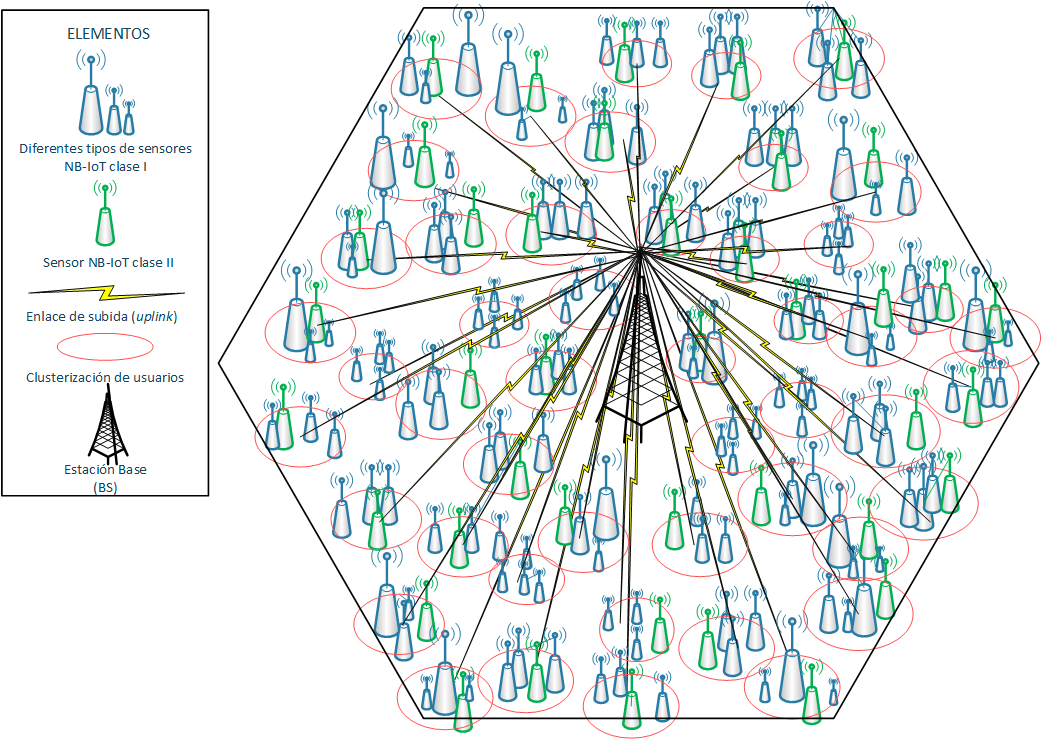
\includegraphics[scale=.7]{Figures/Escenario mIoT unicelda}
\decoRule
\caption[Escenario mIoT unicelular aproximado a simular, usando agrupaciones de 4 dispositivos]{Escenario mIoT unicelular aproximado a simular, usando agrupaciones de 4 dispositivos}
\label{fig:EscenarioMTC}
\end{figure}

Para planear un modelo de sistema valido y coherente se contempló la incorporación de algunos parámetros generales de diseño revisados en artículos [25-27]. La \textit{Tabla~\ref{tab:ParametrosGral}} describe el conjunto de parámetros de la simulación.

Algunos parámetros seguirán las características de las mediciones que se hicieron para validar el modelo CI, en \parencite{Sun2016}. Las mediciones se realizaron en Vestby, Aalborg, Dinamarca, en las bandas de frecuencia de 2, 10, 18 y 28 GHz en marzo. Vestby representa una típica ciudad europea de tamaño mediano con construcciones y anchos de calle regulares, que son de aproximadamente 17 m (cinco pisos) y 20 m, respectivamente. Para el escenario UMi, la antena de la estación base (BS) está a la altura de la azotea, típicamente a 10 m más o menos del suelo, como se define en \parencite{Sun2016}, son antenas direccionales que emplean la formación de haz.

\begin{table}
\caption{Parámetros de la simulación a nivel de sistema}
\label{tab:ParametrosGral}
\centering
\begin{tabular}{|m{6cm}|p{10cm}|} \\ 
\textbf{Parámetro} & \textbf{Valor} \\ 
\textit{Diseño celular}  & \footnotesize{ uni-celda } \\ \hline 
\textit{Radio de celula}  & \footnotesize{ 500m } \\ \hline 
\textit{Movilidad de UEs}  & \footnotesize{ Nula - 0km/h } \\ \hline 
\textit{Distribución de UEs } & \footnotesize{ Procesos puntuales de Poisson } \\ \hline 
\textit{Modelo de canal de propagación `Path Loss' } & \footnotesize{ Modelo CI\newline $L^{CI}_p(f,d)_{\left[dB\right]}=32.4+\ 10\ n{\ log}_{10}\left(\frac{d}{d_0}\right)+{\ 20\ log}_{10}\left(d_0\right)+{20\ log}_{10}\left(f\right)+x^{CI}_{\sigma .}$ } \\ \hline 
\textit{Numero de antenas BS } & \footnotesize{ 1 } \\ \hline 
\textit{Numero de antenas UE } & \footnotesize{ 1 } \\ \hline 
\textit{Potencia de transmisión  de nodos IoT } & \footnotesize{ 23 dBm } \\ \hline 
\textit{Densidad de Ruido Térmico} & \footnotesize{ -174 dbm/Hz } \\ \hline 
\textit{Frecuencia de operación}  & \footnotesize{ En banda y guarda de banda LTE, estándar\newline Principalmente de 2 a 6 GHz } \\ \hline 
\textit{Espacio entre sub-portadora}  & \footnotesize{ 3.75kHz } \\ \hline 
\textit{Ancho de banda del sistema para un PRB (BW) } & \footnotesize{ 180 KHz } \\ \hline 
\textit{Uplink (UL) } & \footnotesize{ 3.75kHz para unitono\newline 15kHz para multitono } \\ \hline 
\textit{Tasa de datos máxima} & \footnotesize{ UL: 20kbps unitono\textit{singletone }} \\  
\end{tabular}
\end{table}

%----------------------------------------------------------------------------------------
%	SECTION 
%----------------------------------------------------------------------------------------

\section{}

\myworries{TODO: Agregar nuevos diagramas de acuerdo con la simulación de eventos discretos}\newline


